\chapter{Sampling}%
\label{chap:sampling}

	The designed architecture uses a sampling approach for path planning. Path
	planning was first investigated in two dimensions before generalising to the
	spatial case. The sampling algorithm used is a variant
	of the well-known \gls{rrt}
	algorithm~\cite{bib:planning:rapidly-exploring_random_trees_a_new_tool_for_path_planning}.

	\section{Overview of Planning Steps}

		As an initial overview, Figure~\ref{fig:path_planning_in_2d} shows the
		different planning stages for the planar case. The orange shapes
		represent obstacles that must be avoided. The green dot is the start
		pose of the end-effector, and the red dot is its final pose. For
		simplicity, the end-effector is not drawn in these images. The top-left
		image shows the construction of a topological graph representing
		possible collision-free paths of the end-effector. The top-right image
		shows the output of a graph-search to obtain a feasible path after the
		graph has been built. The bottom-left shows the output of several
		post-processing steps that optimise and simplify the found path.
		Finally, the bottom-right image shows the effect of smoothing the
		corners of the simplified path.

		\begin{figure}[htb]
			\centering
				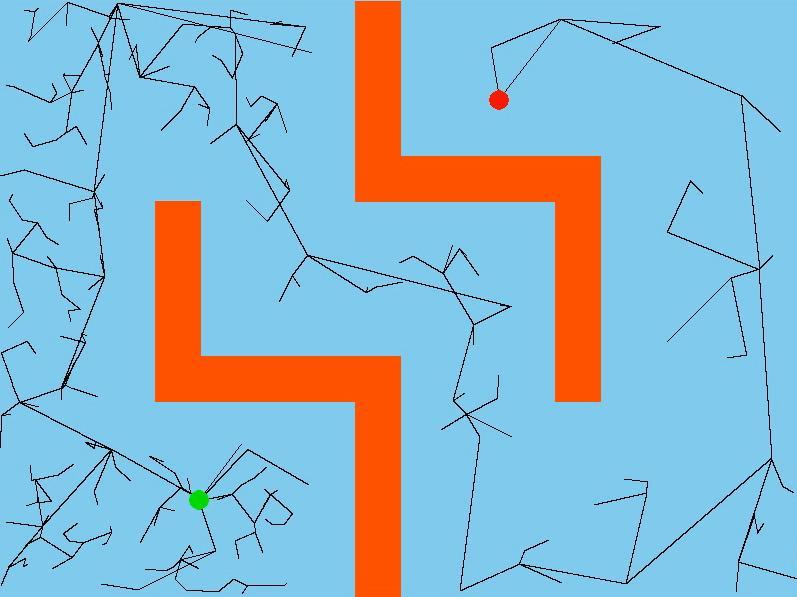
\includegraphics[width=0.5\textwidth]{2d_search_1}%
				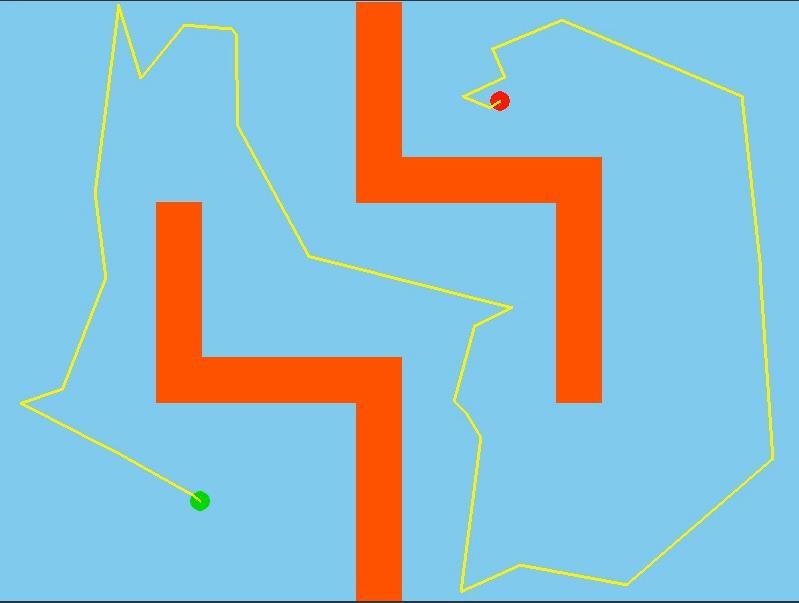
\includegraphics[width=0.5\textwidth]{2d_search_2}\\
				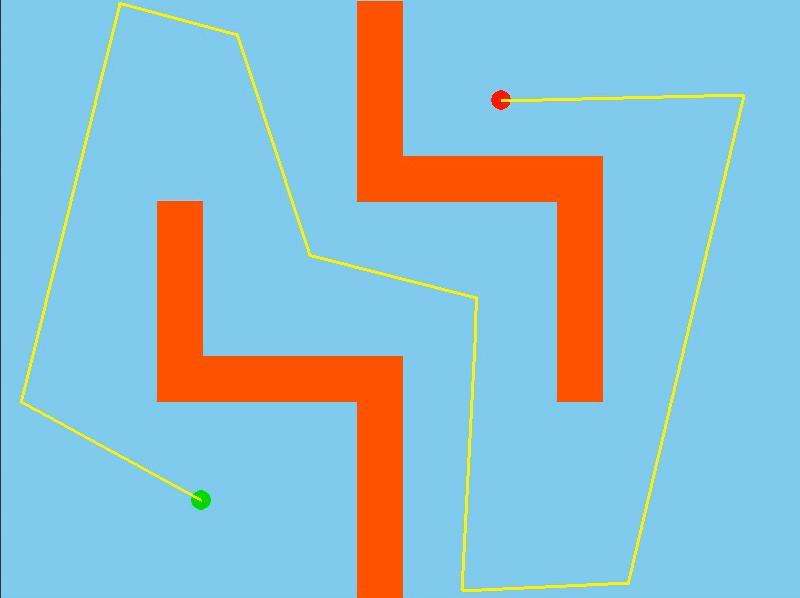
\includegraphics[width=0.5\textwidth]{2d_search_3}%
				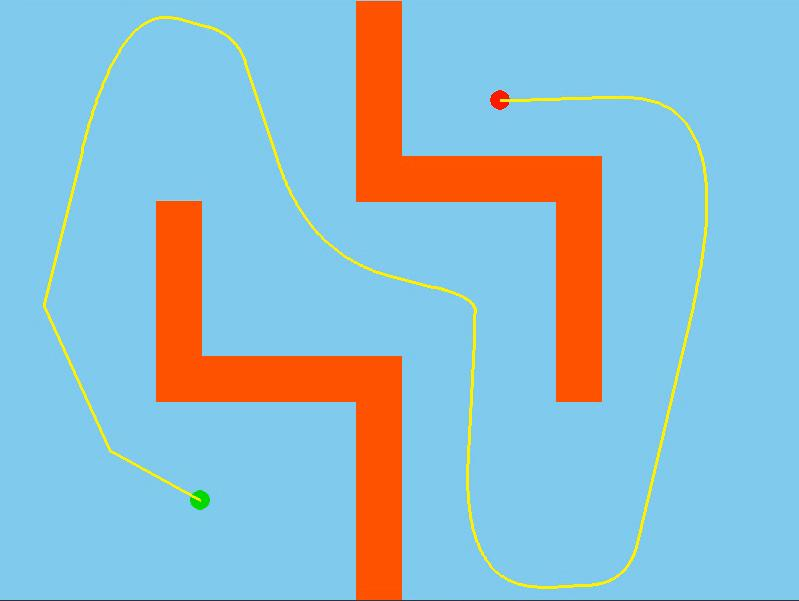
\includegraphics[width=0.5\textwidth]{2d_search_4}
			\caption{Path Planning in 2D}
			\label{fig:path_planning_in_2d}
		\end{figure}

		The current chapter discusses the generation of the topological graph
		and subsequent graph search in the top row of
		Figure~\ref{fig:path_planning_in_2d}. Chapter~\ref{chap:path_processing}
		discusses the post-processing phases shown in the bottom row of the
		figure.  Both chapters discuss these procedures for the general case in
		$\specialEuclideanGroup{3}$.

	\section{Sampling Algorithm Overview}%
\label{sec:algorithm_overview}

	% Due to the topology of the class of \gls{cdpr} considered, the sampling
	% algorithm does not need to sample in configuration space, but may instead
	% sample poses directly. This is due to the fact that there is a one-to-one
	% correlation between end-effector pose and robot configuration.

	The first step of the algorithm is to build a topological graph
	$\topologicalgraph$ whose vertices contain collision-free end-effector
	poses. The edges of the graph represent paths between these poses that are
	also free of collision.  After $\topologicalgraph$ is built, a path
	$\pathsym$ is found that connects the start pose $\pose_{\initial}$ to the
	final pose $\pose_{\final}$ by taking into account a custom-defined distance
	function $\dist(\pose_1, \pose_2)$ between two neighbour poses in
	$\topologicalgraph$. A schematic representation is shown in
	Figure~\ref{fig:path_search}. The left side of the figure shows a
	representation of $\topologicalgraph$ in configuration space, whereas the
	right side shows an as-of-yet inefficient path from the start to the goal.

	\begin{figure}[hb]
		\centering
		\def\svgwidth{\columnwidth}
		\import{res/img/}{path_search.pdf_tex}
		\caption{Initial Path Search}%
		\label{fig:path_search}
	\end{figure}


	The pose $\pose$ of the robot $\robot$ is described as a translation
	vector $\transvec$ combined with a quaternion $\quaternion$:

	\begin{equation}
		\pose = (\transvec, \quaternion)
	\end{equation}

	Furthermore, the algorithm defines a graph $\topologicalgraph$ of poses.
	During each iteration, the algorithm samples a new pose,
	$\pose_{\indexi}$ such that:

	\begin{equation}
		\robot(\pose_{\indexi}) \not\in
		\configurationspace_{\obstacleregion}
	\end{equation}

	and attempts to add it to the graph:

	\begin{equation}
		\topologicalgraph_{\indexi + 1} \leftarrow
			\topologicalgraph_{\indexi} \cup \pose_{\indexi}
	\end{equation}

	in such a way that:

	\begin{equation}
		\exists \pose_{\indexj} \in \topologicalgraph_{\indexi}
			\quad\suchthat\quad
			\vecline{\pose_{\indexi}}{\pose_{\indexj}} \notin
			\configurationspace_{\obstacleregion}
	\end{equation}

	This last line states that the new sampled pose may be connected to some
	other pose already in the graph in such a way that the path connecting
	the two poses is free of collisions.

	At the same time, at each iteration, the algorithm attempts to add the
	goal pose $\pose_{\goal}$ to $\topologicalgraph$. If this is
	successfully executed, then a path has been found and the algorithm
	terminates. A high-level overview of the algorithm can be found in
	Algorithm~\ref{alg:sampling_planning_overview}.

	\begin{algorithm}[ht]
		\caption{Sampling Planning Overview}%
		\label{alg:sampling_planning_overview}
		\begin{algorithmic}[1]
			\Procedure{Sample\_Search}{$\robot, \obstacle_1, \ldots, \obstacle_n$}
				\State{}$\topologicalgraph = \emptyset \cup \pose_{\initial}$
				\While{$\pose_{\goal} \notin \topologicalgraph$}
					\Repeat{}
						\State{}$\pose_\text{sampled} \leftarrow
						\code{sample\_pose}$\label{alg:sampling_planning_overview:sample_pose}
					\Until{$\robot(\pose) \notin \configurationspace_{\obstacleregion}$}
					\State{}
						\(
							\pose_{\text{neighbour}} =
							\argmin_{\pose_{\indexi} \in
							\topologicalgraph}\dist(\pose_\text{sampled}, \pose_{\indexi})
						\)
					\State{}$\pose_\text{new} =
						\code{farthest\_collision\_free\_point}(\pose_{\text{sampled}},
						\pose_{\text{neighbour}})$\label{alg:sampling_planning_overview:farthest_collision_free_point_sampled}
					\State{}$\code{connect}(\pose_\text{neighbour},
						\pose_\text{new})$
					\State{}$\pose_\text{new} =
						\code{farthest\_collision\_free\_point}(\pose_{\text{new}},
						\pose_{\text{\goal}})$\label{alg:sampling_planning_overview:farthest_collision_free_point_goal}
					\If{$\pose_\text{new} == \pose_{\goal}$}
						\State{}$\code{connect}(\pose_{\goal},
							\pose_\text{new})$
					\EndIf{}
				\EndWhile{}
			\EndProcedure{}
		\end{algorithmic}
	\end{algorithm}

	\section{Sample Strategy}%
\label{sec:sample_strategy}

	Line~\ref{alg:sampling_planning_overview:sample_pose} of
	Algorithm~\ref{alg:sampling_planning_overview} samples a pose from the
	configuration space of the robot in the following manner:

	\begin{enumerate}

		\item

			A translation vector $\transvec$ is drawn from a normal
			distribution such that:
			\label{item:sample_strategy:translation}

			\begin{enumerate}

				\item

					The median of the distribution is the centre of the
					workspace.

				\item

					The edges of the workspace are three standard deviations
					away from the median.
			\end{enumerate}

		\item

			An angle $\theta$ is drawn from a normal distribution with
			median $\pi/2$ and standard deviation $\pi/6$.

			\label{item:sample_strategy:angle}

		\item

			A quaternion is built from the formula:

			\begin{equation}
				\quaternion = 0\vec{i} + \sin(\theta/2)\vec{j} + 0\vec{k} +
					\cos(\theta/2)
			\end{equation}

			\label{item:sample_strategy:quaternion}

			%This produces a rotation of angle $\theta$ around the $y$
			%axis.\todo{explain that y axis is pointing up}

		\item

			The pose $\pose = (\transvec, \quaternion)$ is returned.

	\end{enumerate}

	\subsection{Justification of Sampling Strategy}%
	\label{sec:justification_of_sampling_strategy}

		\glspl{cdpr} are more likely to have a higher capacity margin towards
		the centre of their workspace. This led to the decision to use a normal
		distribution to sample translations as described in
		Item~\ref{item:sample_strategy:translation} above. In doing so, the
		sampling algorithm has a higher probability to choose translations
		closer to the centre of the workspace, thereby increasing the average
		stability of the trajectory found.

		Items~\ref{item:sample_strategy:angle}
		and~\ref{item:sample_strategy:quaternion} in the list above generate a
		rotation $\theta$ around the $y$-axis. The reason that rotations are
		only drawn around the $y$ axis is two-fold. The first reason is that
		experimentation has shown that the architecture performs faster when
		only drawing rotations around a single axis. This is because, by
		removing two rotational axes, the search space is reduced by two
		dimensions. The second reason is that, by only drawing rotations around
		the $y$ axis, the robot is guaranteed to be upright during its
		trajectory. This produces simpler trajectories, as generating completely
		random quaternions would have the robot change its orientation
		unpredictably.

		The mean and standard deviation as defined in
		Item~\ref{item:sample_strategy:angle} are chosen such that 99.7\% of
		the sampled rotations lie within the range $\theta \in [0, \pi]$.
		The effect of using a uniform distribution within this range instead
		of the distribution of Item~\ref{item:sample_strategy:angle} was
		also investigated. This, however, was deemed an inefficient
		approach, as the end-effector was found to have a tendency to
		unnecessarily swing back and forth around the $y$-axis as it
		progressed through its trajectory. By instead biassing the
		end-effector's orientation towards a certain median position, the
		need for a post-processing operation to simplify the orientation's
		progression was significantly reduced.

		Following this approach, given an arbitrary start and end pose, the
		architecture finds a path through several poses in such a way that,
		while moving from the start pose to the first sampled pose, the
		robot is turned upright. Then, while in the middle of its
		trajectory, the robot stays upright. Finally, as the robot
		approaches its final pose, it performs any required arbitrary
		rotations to reach the desired goal pose. This is shown
		schematically in Figure~\ref{fig:pose_sampling}.

		\begin{figure}[hb]
			\centering
			\def\svgwidth{\columnwidth}
			\import{res/img/}{pose_sampling.pdf_tex}
			\caption{Pose Sampling}%
			\label{fig:pose_sampling}
		\end{figure}

	\subsection{Improving the Sampled Capacity Margin}%
	\label{sec:improving_the_sampled_capacity_margin}

		While the sampling strategy in
		Algorithm~\ref{alg:sampling_planning_overview} will find a
		collision-free path, the path may be suboptimal in terms of the capacity
		margin. The capacity margin may be improved as part of a post-processing
		step as explained in Section~\ref{sec:increasing_the_capacity_margin}.
		However, relying on pure post-processing can be expensive. A small
		modification to Algorithm~\ref{alg:sampling_planning_overview} is
		therefore proposed here.

		The idea is to sample poses as before, but then immediately after
		Line~\ref{alg:sampling_planning_overview:sample_pose} in
		Algorithm~\ref{alg:sampling_planning_overview} move them in the
		direction of increasing capacity margin $\capacitymargin$ according to:

		\begin{equation}
			\pose \gets \pose +
				\gain\frac
				{%
					\nabla\capacitymargin
				}
				{%
					\norm
					{%
						\nabla\capacitymargin
					}
				}
			\label{eq:improve_sampled_capacity_margin}
		\end{equation}

		This operation is fairly cheap. Therefore, $\gain$ is kept small and
		Equation~\ref{eq:improve_sampled_capacity_margin} is performed
		repeatedly on the sampled pose $\pose$. This can be seen as taking
		random samples from the configuration space, and then ``sliding'' them
		along the curve defining the direction of increasing capacity margin for
		some predefined distance.

		Due to the shape of the capacity margin polytope, if all samples have a
		favourable capacity margin, then the entire path through these poses
		will also have a good capacity margin.


	\section{Path Checking}%
\label{sec:path_checking}

	\begin{sloppypar}

		There is no guarantee that a sampled pose $\pose_\text{sampled}$ can
		be connected directly to its nearest neighbour
		$\pose_\text{neighbour} \in \topologicalgraph$.
		Figure~\ref{fig:nearest_neighbour} shows one such case. In the figure,
		the green dot represents the last sampled pose. There exists no
		straight-line collision-free path from its nearest neighbour, indicated
		by the red line.

		\begin{figure}[hb]
			\centering
			\def\svgwidth{0.75\columnwidth}
			\import{res/img/}{nearest_neighbour.pdf_tex}
			\caption{Invalid nearest neighbour}%
			\label{fig:nearest_neighbour}
		\end{figure}

		For this reason, the calls to
		$\code{farthest\_collision\_free\_point}$ in lines
		Lines~\ref{alg:sampling_planning_overview:farthest_collision_free_point_sampled}
		and~\ref{alg:sampling_planning_overview:farthest_collision_free_point_goal}
		of Algorithm~\ref{alg:sampling_planning_overview} attempt to
		guarantee that there is no collision between these points.

	\end{sloppypar}

	This is done by discretising points between $\pose_\text{neighbour}$ and
	$\pose_\text{sampled}$ in a straight-line fashion and returning the
	point farthest from $\pose_\text{neighbour}$ before any collision is
	detected. This is summarised in
	Algorithm~\ref{alg:farthest_collision_free_point}.

	\begin{algorithm}[ht]
		\caption{Farthest Collision Free Point}%
		\label{alg:farthest_collision_free_point}
		\begin{algorithmic}[1]
			\Procedure{Farthest\_Collision\_Free\_Point}{$\pose_1, \pose_2$}
				\State{}$\code{dist\_to\_travel} = \dist(\pose_1, \pose_2)$
				\State{}$\code{dist\_travelled} = 0$
				\State{}$\pose_\text{intermediate} = \pose_1$
				\State{}$\pose_\text{prev-intermediate} = \pose_1$
				\While{$\code{dist\_travelled} < \code{dist\_to\_travel}$}
					\State{}
						\(
							\pose_\text{intermediate} =
							\pose_1 +
							\code{dist\_travelled}/\code{dist\_to\_travel}
							(
								\pose_2 - \pose_1
							)
						\)
					\If{\robot($\pose_\text{intermediate}) \in \configurationspace_{\obstacleregion}$}
						\State{}$\pose_\text{intermediate} =
							\pose_\text{prev-intermediate}$
						\State{}break
					\EndIf{}
					\State{}$\code{dist\_travelled} =
						\code{dist\_travelled} + \Delta\configuration$
					\State{}$\pose_\text{prev-intermediate} =
						\pose_\text{intermediate}$
				\EndWhile{}
				\If{$\code{dist\_travelled} > \code{dist\_to\_travel}$}
					\State{}return $\pose_2$
				\EndIf{}
				\State{}return $\pose_\text{intermediate}$
			\EndProcedure{}
		\end{algorithmic}
	\end{algorithm}

	The term $\Delta\configuration$ in
	Algorithm~\ref{alg:farthest_collision_free_point} is an increment that
	determines the resolution at which paths are checked. Its value must be
	chosen such that the algorithm executes quickly, but does not jump over
	obstacles. Its value essentially determines a sphere of radius
	$\Delta\configuration$ around every sampled pose $\pose$ within which it
	is not certain if there is a collision or not.

	% This uncertainty is negated by creating virtual obstacles that are
	% larger than the actual obstacles by a value
	% greater than $\Delta\configuration$. That way, if there is a collision
	% in the uncertain points between $\pose_1$ and $\pose_2$, it will be a
	% collision with a virtual obstacle, but not with the real obstacle.
	% \todo{When this is implemented, discuss it better}

	\section{Distance Measure}%
\label{sec:distance_measure}

	Both Algorithm~\ref{alg:sampling_planning_overview}
	and~\ref{alg:farthest_collision_free_point} require to measure the
	distance between two poses, $\dist(\pose_1, \pose_2)$. This poses a
	problem, however, as a pose is a member of the special euclidean group,
	$\pose \in \specialEuclideanGroup{3}$. There is no one way to measure
	distances in this set and an arbitrary measure is often required. There
	is also the problem that the units used for rotations and translations
	differ.

	Several different measures are often used in these cases. One is to
	simply define the distance as the translational distance between two
	poses:

	\begin{equation}
		\dist(\pose_1, \pose_2) =
			\norm{%
				\pose_2.\transvec - \pose_1.\transvec
			}
		\label{eq:euclidean_distance}
	\end{equation}

	\todo{Add radius of gyration discussion here}

	This thesis proposes to instead measure distances in cable-space. This
	has the following advantages:

	\begin{itemize}

		\item

			Dimensionally homogeneous. Since each pose is related directly
			to the length of the cable-space vector, both the translation
			and orientation of a pose can be measured using meters.

		\item

			Direct correlation to actuators. The change in length of the
			cables relates directly to how much the actuators have to act on
			the cables. Using the cable-space vector as a distance measure
			means that the distance exactly encodes the amount of actuation
			required to move from one pose to another.
			\todo{wording}

	\end{itemize}

	The cable-space vector, $\cablelengths$, can be found from the indirect
	geometric model of the \gls{cdpr}:

	\begin{equation}
		\cablelengths = \invgeometricmodel(\pose)
	\end{equation}

	The distance function is then taken as:\todo{make sure this is correct,
	and implement it in the code}

	\begin{equation}
		\dist(\pose_1, \pose_2) =
			\norm{%
				\invgeometricmodel(\pose_2) - \invgeometricmodel(\pose_1)
			}
		\label{eq:distance_measure}
	\end{equation}

	\subsection{Incorporating the Capacity Margin}%
	\label{sec:incorporating_the_capacity_margin}

		It may be useful to include the value of an index, such as the capacity
		margin, in the distance calculation. For such cases
		Equation~\ref{eq:distance_measure} may be modified to obtain:

		\begin{equation}
			\dist_{\pathsym}(\pose_1, \pose_2) =
				-\gain_{\capacitymargin}
				\frac%
				{%
					\int_0^1 \capacitymargin(\pathsym(\timenorm))\der\timenorm
				}
				{%
					%\int_{\pathsym} \der\pose
					\capacitymargin(\pose_2) - \capacitymargin(\pose_1)
				}
				+
				(1 - \gain_{\capacitymargin})
				\norm{%
					\invgeometricmodel(\pose_2) - \invgeometricmodel(\pose_1)
				}
				\label{eq:distance_measure_capcity_margin}
		\end{equation}
		\todo{This has not yet been implemented in code}
		\todo{dimensionally homogeneous?}

		Here
		\(
			\dist_{\pathsym}
		\)
		measures the distance along the path $\pathsym$ and
		\(
			\gain_{\capacitymargin} \in [0, 1]
		\)
		is a weighting factor that weighs the relative importance of the change
		in capacity margin for a longer path to the straight-line distance
		between two poses.

		The negative sign in front of the integral in
		Equation~\ref{eq:distance_measure_capcity_margin} is due to the fact
		that a path for which the capacity margin is higher should be considered
		more advantageous and therefore shorter.

		The integral in Equation~\ref{eq:distance_measure_capcity_margin} is
		expensive to evaluate repeatedly during the path-planning phase. As
		such, it is instead approximated using a...
		\todo{when implemented, flesh out the following paragraph}


